\tightsection{Background and Motivation}



\jc{need a better transition from the general idea of prediction-centric to video-specific optimization.}

\tightsubsection{Need of quality prediction}

\myparasum{Today's video quality} Previous research has confirmed the impact of quality on user experience that users are quite sensitive to buffering and high startup latency, and prefer higher bitrate content. Moreover, it also has been confirmed that today's end user experience is far from perfect and quality optimization is needed\cite{sigcomm12,conext13}.

\myparasum{What decisions can be made for a video session} A typical way of Internet video delivery is that during a video session, the video player streams the video object from a server by sequentially downloading chunks in a progressive download fashion or periodically. In this context, today's video delivery infrastructure provides two control knobs -- {\it CDN} in which the server is located, {\it bitrate} in which the object is encoded -- for a video player to adapt against changes in network condition and resource availability. The CDN and bitrate can be chosen from a pre-determined set of options and can be switched at any point during a session. Readers may refer to~\cite{conext12} for more details. 

\myparasum{Previous research has shown prediction is necessary} Therefore, a fundamental challenge for quality optimization is to make the best decision (i.e., CDN, bitrate) for each session. In this context, previous research \cite{sigcomm12,conext13} has shown (1) significant spatial diversity in CDN performance \footnote{CDN performance means the overall video quality that viewers experience if the video is streamed from it.} and availability across different geographical regions and ISPs; (2) substantial temporal variability in the CDN performance and client-side network performance; and (3) that causes of quality issues can be rooted in various attributes of a session (e.g., content provider, player implementation, or a combination). These results have implied that there is no globally best decision which performs better than others for most sessions and for most of time, and therefore, the best decision for any session should be made by predicting the video quality if each decision were to be used. 

\myparasum{Approaches towards quality prediction} In order to accurately predict the outcome of each decision, one approach to model the quality changes of decision. However, such quality prediction model can be costly to maintain for each session and highly complex given the complexity of the delivery infrastructure itself. Alternatively, we argue that a data-driven approach that leverages the power of massive measurements from clients is more practical and as we will demonstrate later, can predict quality accurately with proper algorithms.

\myparasum{Organization of rest of this section} In the rest of the section, we will describe our dataset for trace-driven analysis, and then present preliminary statistics to motivate that data-driven accurate prediction is also feasible by sharing information and quality measurements from clients. 

\tightsubsection{Dataset (mostly copied from CoNEXT)}
\label{subsec:dataset}

\myparasum{Dataset overview} Our dataset is based on client-side measurements of video quality from over \fillme million sessions or views (both successful and failed) over a duration of \fillme days. The data was generated via client-side player instrumentation that monitors the state of player and network condition, collects the statistics regarding the observed video quality (e.g., rebuffering ratio, chosen bitrate) and session attributes (e.g., ASN, chosen CDN, player type). These collected information will be sent back to the backend so that we can maintain up-to-date quality and attribute information of each observed session.

\myparatight{Quality sample} The basic unit in our dataset is a {\it quality sample}\jc{quality sample is just more expressive way of SessionInterval.}. A quality sample represents a user viewing a video on one of our affiliates' sites for a fixed interval of time\jc{is SessionInterval always for one minute in current implementation?}. Each quality sample is associated with four fields -- session ID, attributes, timestamp and quality metrics. 

\myparatight{Attributes} There are \fillme attributes that we observe and collect at client-side:

\begin{packedenumerate}
\item \emph{ASN:} The Autonomous System Number (ASN) that the client IP belongs
 to. Note that a single ISP (e.g., Comcast) may own different ASNs both
 for management and business reasons. We focus on the ASN as it is more fine-grained
 than the ISP granularity.  We observe in aggregate \fillme unique ASNs
  spanning multiple countries.

\item \emph{CDN:}   In total, we observe
\fillme unique CDNs spanning popular CDN providers as well as several in-house and
ISP-run CDNs. (Some providers use proprietary CDN switching logic; in
this case we pick the segment of the session with the CDN used for the longest
duration.)

\item \emph{Content provider (Site):} This is the specific affiliate content
provider from which the client requested some content. We have  \fillme content
providers that span different genres of content.  We use the terms site and
content provide interchangeably.

\item \emph{VoD or Live:} Video  content  falls in one
 of two categories: video-on-demand (VoD) or Live.  We use a binary indicator to
 see if the particular content was a Live event or a VoD video.

\item \emph{Player type:} We see diverse  players such as  Flash, Silverlight,
and HTML5.

\item \emph{Browser:} We see diverse client browsers including Chrome, Firefox,
MSIE, and Safari.

\item \emph{Connection type:} Finally, we  have the type of
access network connection such  as
 mobile/fixed wireless, DSL, fiber-to-home. These annotations come from third party services~\cite{quova}.

Notice that decision (i.e., CDN, bitrate) is also counted as attributes in quality samples.

\end{packedenumerate}

\myparatight{Quality metrics} We focus on four industry-standard video quality metrics that have been shown to be critical for measuring user engagement~\cite{sigcomm11}:
\begin{packedenumerate}
\item \emph{Buffering ratio:}  Given a video session of duration $T$~seconds,
if the player spent $B$~seconds in buffering (i.e., waiting for the player
 buffer to replenish midstream, the buffering ratio is defined as
 $\frac{B}{T}$. Prior work has shown that buffering ratio is a key metric
 that impacts user engagement~\cite{sigcomm11}.
\item \emph{Join time:}  This is the time taken for the video to start playing
 from the time the user clicks on the ``play'' button on the player.
 While join time may not directly impact the amount of a specific video viewed,
 it does have long term effects as it reduces the likelihood of repeated
visits~\cite{sigcomm11,akamai-imc12}.
\item \emph{Average bitrate:} Many video players today support adaptive bitrate
selection and midstream bitrate switching to adapt to changing bandwidth
availability. The average bitrate of a session is simply the time-weighted
average of the bitrates used in a given session. (Bitrate refers to the video playback rate, rather than throughput or download rate.)
\item \emph{Start failures:}   Some sessions may not even start playing the
video; either the content is not available on the CDN server or the CDN is
under overload or other unknown reasons. We mark as a session as a join failure
if no content was played during this session.\footnote{Start failures are
reported by the client-side measurement module that sends a ``heartbeat'' on
the player status.}
\end{packedenumerate}

\myparatight{Timestamp} The timestamp is the system at backend when the sample is received from client. There are two sources of measurement noise in our implementation: (1) The backend system time is different from when the sample is actually collected. (2) Some quality metrics (e.g., join time) reflect the quality at the beginning of a session of rather than the current time point. \jc{The impact of each of these noise should be discussed later.}

\tightsubsection{GO system overview}

\myparasum{We have built a real system} The richness of our dataset allows us to make more informed decisions. We have implemented a working prototype called Video Global Optimization (GO) to realize this goal and to actually improve video quality in the wild.  Here we describe its architecture for gathering data and making decisions; the remainder of this paper will focus on the mapping from data to decisions via prediction.

\myparasum{Highlevel components} Physically, in order to collect statistics from client and make decision in a centralized manner, GO has two parts: instrumentation code running within players during the cause of a video session at client-side, and GO backend running in publicly available clusters for centralized processing. Logically, there are three components of GO system (see Figure \fillme). 

\myparatight{Quality sample collection} To collect feedback from client-side video sessions, the instrumentation code monitors the state of player and network condition, summarizes them in the form of quality samples (see details in \Section~\ref{subsec:dataset}) and send the quality samples back to GO backend for storage. Quality samples are then stored in a Hadoop File System for storage. \jc{in reality, the raw input from client is in log format of heartbeat, and later processed into quality samples by the backend. we may decide whether to expose it in scalability section.}

\begin{figure}[h!]
\centering
 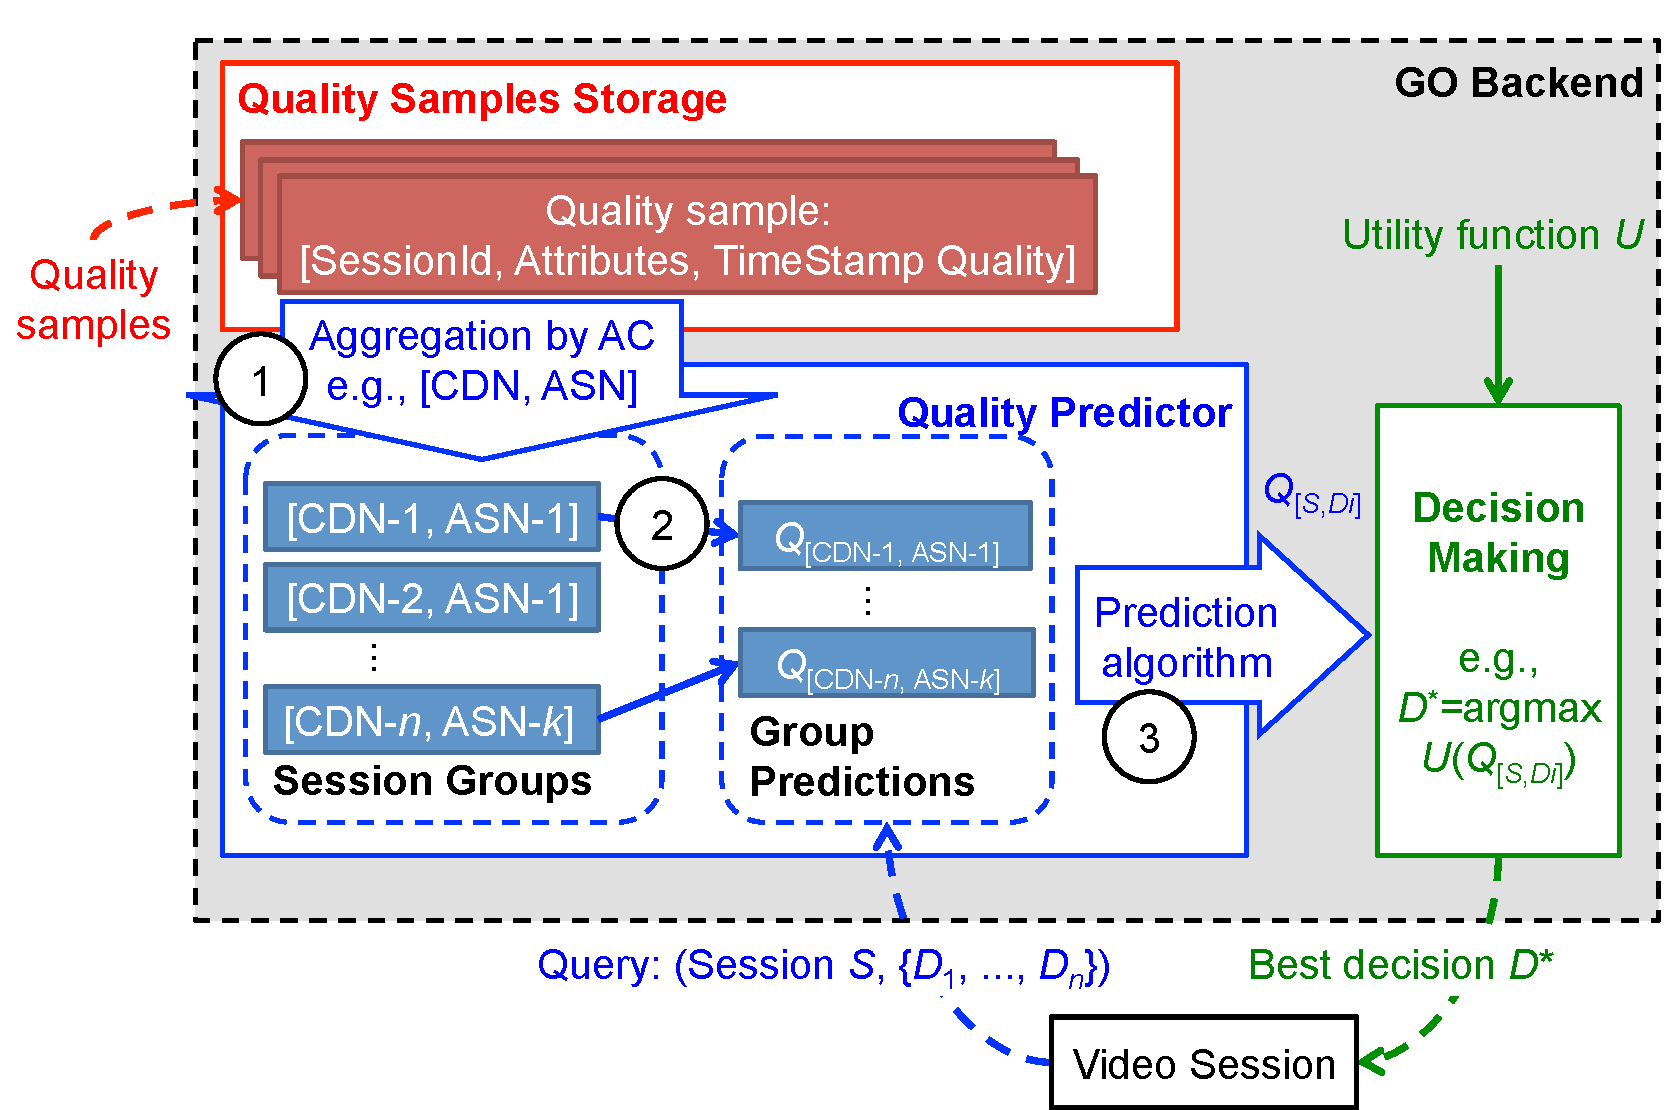
\includegraphics[width=0.5\textwidth] {figures/backend.pdf}
\tightcaption{Schematic overview of GO backend.}
\label{fig:backend}
\end{figure}

\myparatight{Quality prediction} Quality samples are mapped to predictions about quality outcomes of future sessions for each possible decision.  We postpone discussion of the details of this mapping for now.  For efficiency reasons, this step cannot rely on all available quality samples; they must be sampled or aggregated in some fashion.

\myparatight{Decision making} A simple procedure is used to decide on the optimal CDN or bitrate for a video session: A predicted quality metric is computed for each possible decision, and then the decision maximizing predicted quality is taken.  Since there are multiple quality metrics, they must be combined into a single figure of merit via a \emph{utility function}.  For example, a utility function may return a linear combination of several quality metrics.
